\documentclass[11pt]{beamer}
\usetheme{CambridgeUS}
\usepackage[utf8]{inputenc}
\usepackage[english]{babel}
\usepackage{amsmath}
\usepackage{amsfonts}
\usepackage{amssymb}
\usepackage{graphicx}
\graphicspath{ {images/} }
\usepackage{color}

\author{Saša Dešić, \underline{Mia Filić} and Renato Filjar}
\title{Determination of origins and destinations
for an O-D matrix based on telecommunication activity records}
\setbeamercovered{transparent} 
\setbeamertemplate{navigation symbols}{} 
%\logo{} 
%\institute{} 
\date{} 
%\subject{} 
\begin{document}

\begin{frame}
\titlepage
\end{frame}

\begin{frame}{•}
	\frametitle{Introduction}
	\begin{figure}
      \centering
    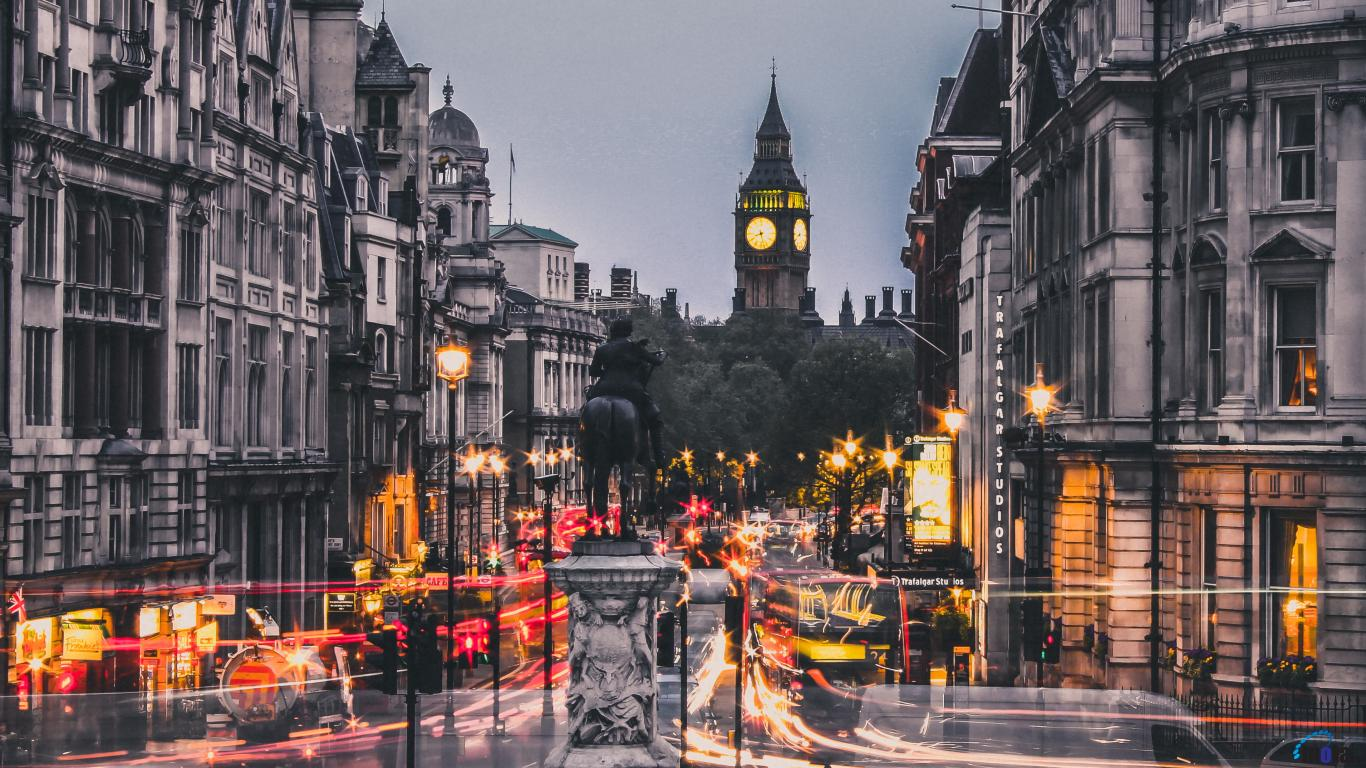
\includegraphics[width=0.7\textwidth]{first}
    
  \end{figure}

\end{frame}

\begin{frame}{•}
	\frametitle{Introduction}
	\begin{figure}
      \centering
    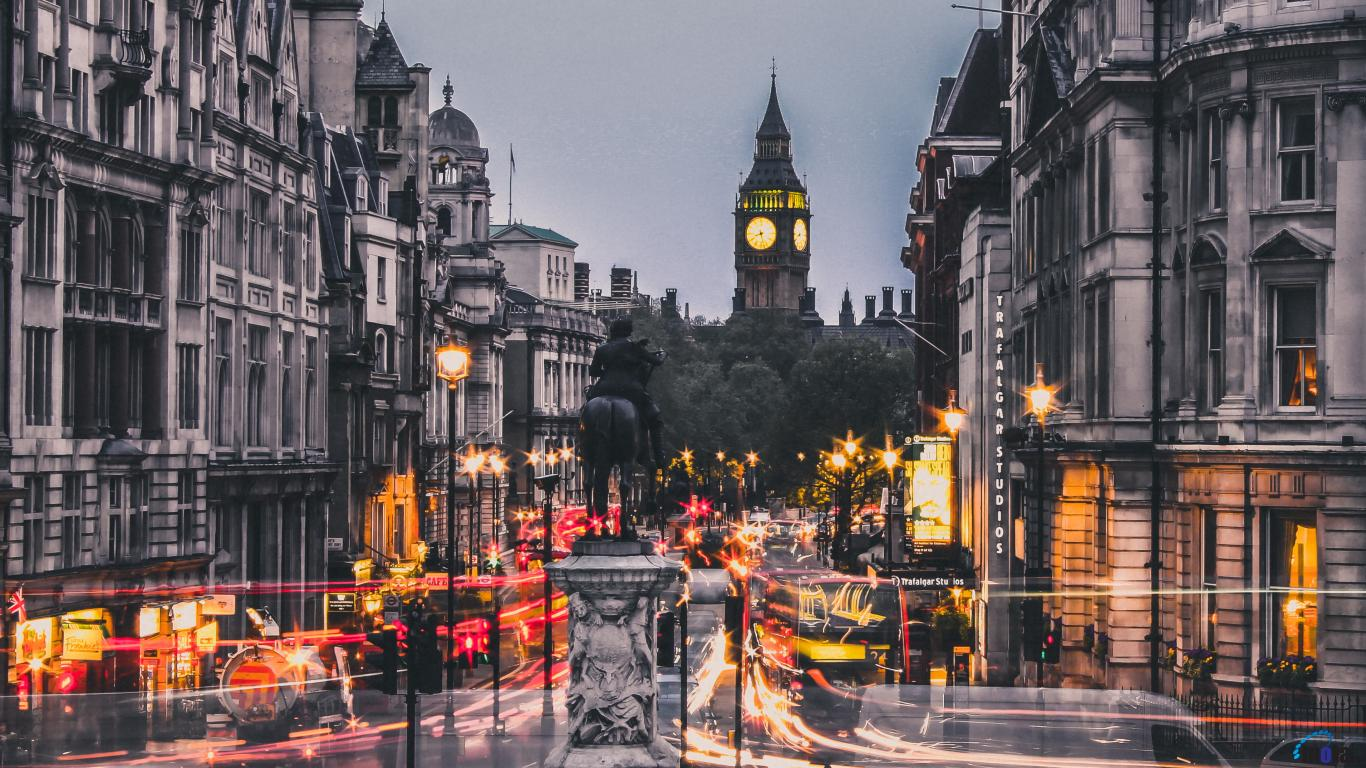
\includegraphics[width=0.7\textwidth]{first}
    
  \end{figure}
  \textbf{How to track OD movemoent?}
\end{frame}

\begin{frame}
   \frametitle{Origin Destination matrix - OD matrix}
   \begin{figure}
      \centering
    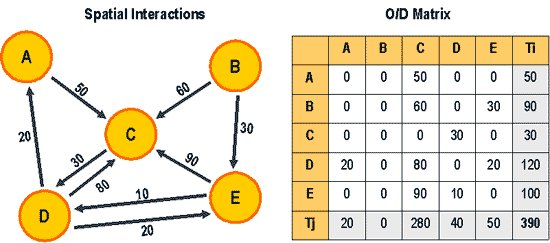
\includegraphics[width=0.7\textwidth]{Odgraph}
    
    \end{figure}

\end{frame}

\begin{frame}
   \frametitle{Origin Destination matrix - OD matrix}
   \begin{figure}
      \centering
    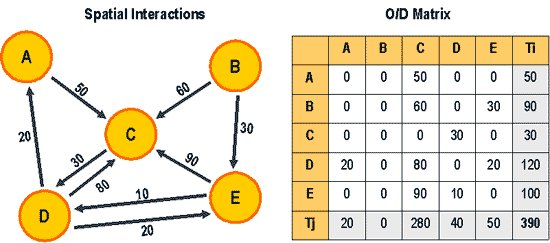
\includegraphics[width=0.7\textwidth]{Odgraph}
    
    \end{figure}
\textbf{How to determine origins and destinations in spartial grid?}
\end{frame}

\begin{frame}
   \frametitle{OD determination}
   \begin{figure}
      \centering
    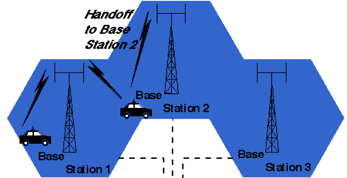
\includegraphics[width=0.7\textwidth]{cells}
    
    \end{figure}

\end{frame}

\begin{frame}
   \frametitle{OD determination}
 \begin{figure}
   \begin{minipage}{0.45\textwidth}
   	\centering
    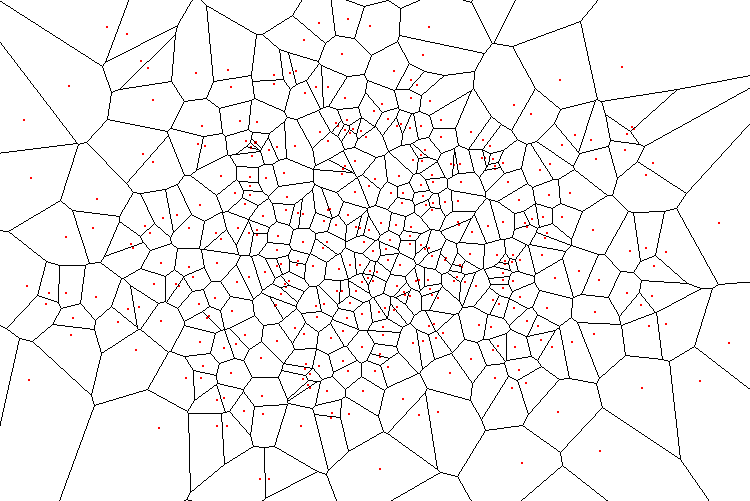
\includegraphics[width=1\textwidth]{voronoi}
   \end{minipage}%
   \begin{minipage}{0.45\textwidth}
   	\centering
    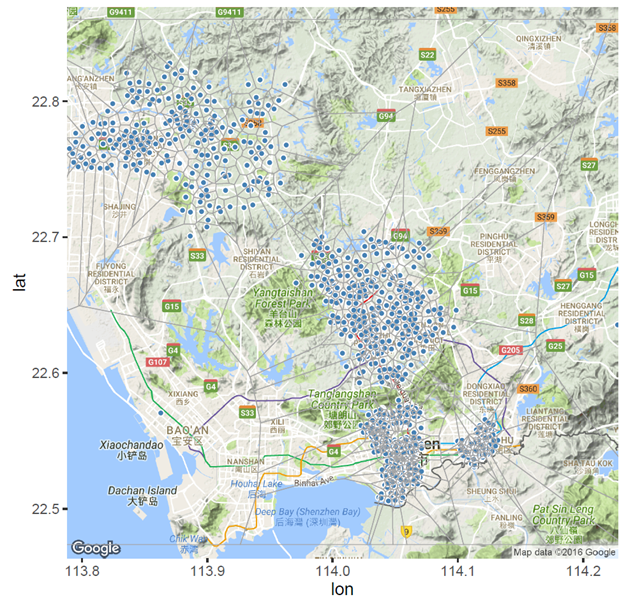
\includegraphics[width=1\textwidth]{voronoi2}
   \end{minipage}
    
  \end{figure}
Why is it better?
\end{frame}

\begin{frame}
   \frametitle{OD determination}
   We used:
 \begin{enumerate}
        \item CDR records
        \item Voronoi tesellation
        \item programming language R
      \end{enumerate}

\end{frame}

\begin{frame}
   \frametitle{OD determination}
   Done:
 \begin{enumerate}
        \item O/D candidates
        \item O/D candidates reduction due to CDRs
      \end{enumerate}
  In future:
 \begin{enumerate}
        \item further O/D candidates reduction using contextual and spatial relation between Voronoi cells seeds and points of socio-economic activities (residental areas, contextual data on shops, 
        concert halls, $\hdots$)
      \end{enumerate}

\end{frame}

\begin{frame}
\frametitle{Questions?}
\centering \LARGE 
  \emph{Thank you for your attention!}\newline
  \newline
\centering \normalsize

Mia Filić, \textcolor{red}{\textit{filicmia@outlook.com}}
\end{frame}

\end{document}